% Agile Orchestrators -- how an AI harness changed scrum work on the Tulip Churn project.
% Custom Rabobank look (override of the latex-presentation default preamble), modelled on the
% team's reference slides: navy/orange title bands, italic blue titles, thin blue line-art paths,
% orange/green rounded boxes on grey panels. Facts come from docs/ai-harness-scrum-log.md,
% the repo (skills, hooks, pyproject.toml) and the GitHub board.
\documentclass[aspectratio=169,10pt]{beamer}
\usepackage[T1]{fontenc}
\usepackage[utf8]{inputenc}
\usepackage{lmodern}
\usepackage[scaled=0.92]{helvet}
\renewcommand{\familydefault}{\sfdefault}
\usepackage{amssymb}
\usepackage{tikz}
\usetikzlibrary{calc,positioning,arrows.meta,shapes.geometric,shapes.misc}

\graphicspath{{./images/}}

% ---------------------------------------------------------------- colours
\definecolor{raboNavy}{HTML}{000099}
\definecolor{raboBlue}{HTML}{0052FF}
\definecolor{raboLine}{HTML}{1C50D7}
\definecolor{raboOrange}{HTML}{FF6600}
\definecolor{raboGreen}{HTML}{03B463}
\definecolor{raboGrey}{HTML}{D9D9D9}
\definecolor{raboPanel}{HTML}{EDEDED}
\definecolor{raboLilac}{HTML}{E9E8F7}
\definecolor{raboPurple}{HTML}{7A2E8E}
\definecolor{raboInk}{HTML}{33334D}
\definecolor{raboMuted}{HTML}{8A8A99}

% ---------------------------------------------------------------- beamer look
\setbeamertemplate{navigation symbols}{}
\setbeamersize{text margin left=0.8cm,text margin right=0.8cm}
\setbeamercolor{normal text}{fg=raboInk,bg=white}
\setbeamercolor{structure}{fg=raboBlue}
\setbeamercolor{alerted text}{fg=raboOrange}
\setbeamertemplate{itemize item}{\tikz[baseline=-0.55ex]\fill[raboOrange] (0,0) circle (1.5pt);}
\setbeamertemplate{itemize subitem}{\tikz[baseline=-0.55ex]\draw[raboBlue] (0,0) circle (1.2pt);}
\setlength{\leftmargini}{1.1em}
\hyphenpenalty=10000
\exhyphenpenalty=10000

\setbeamertemplate{frametitle}{%
  \vspace*{0.30cm}%
  {\color{raboBlue}\itshape\footnotesize\insertframesubtitle\par}%
  \vspace{0.5pt}%
  {\color{raboBlue}\itshape\fontsize{19}{21}\selectfont\insertframetitle\par}%
}

% Default background: page number bottom left, signature + logo bottom right (as on the
% reference slides).
\defbeamertemplate{background}{content}{%
  \begin{tikzpicture}
    \useasboundingbox (0,0) rectangle (16,9);
    \node[anchor=south east,inner sep=0] at (15.72,0.16)
      {
\includegraphics[height=0.70cm]{rabobank-logo}};
    \node[anchor=south east,text=raboBlue,font=\scriptsize\itshape,inner sep=0] at (15.02,0.24)
      {Agile Orchestrators \,\textperiodcentered\, the co\"operative way to scrum with AI};
    \node[anchor=south west,text=raboMuted,font=\tiny,inner sep=0] at (0.3,0.24)
      {\insertframenumber};
  \end{tikzpicture}}
\setbeamertemplate{background}[content]

% Gradient ring used on the title and closing slides (reference slide 2).
\newcommand{\connectorring}[3]{% centre x, centre y, radius
  \foreach \i in {0,...,59}{%
    \pgfmathsetmacro{\a}{215-\i*5.5}%
    \pgfmathtruncatemacro{\p}{100-\i*100/59}%
    \draw[line width=2.6pt,draw=raboOrange!\p!raboPurple]
      ($(#1,#2)+(\a:#3)$) arc[start angle=\a,end angle=\a-5.7,radius=#3];
  }%
  \draw[raboPurple!45,line width=0.5pt] ($(#1,#2)+(250:#3-0.28)$)
    arc[start angle=250,end angle=150,radius=#3-0.28];
}
\newcommand{\ringdot}[5]{% cx, cy, r, angle, label
  \pgfmathtruncatemacro{\q}{max(0,min(100,(215-#4)/3.3))}%
  \filldraw[fill=white,draw=raboOrange!\q!raboPurple,line width=1.3pt]
    ($(#1,#2)+(#4:#3)$) circle (0.17);
  \node[font=\tiny\itshape,text=raboInk,inner sep=1pt,anchor=#4+180] at ($(#1,#2)+(#4:#3+0.25)$) {#5};
}

\defbeamertemplate{background}{title}{%
  \begin{tikzpicture}
    \useasboundingbox (0,0) rectangle (16,9);
    \fill[raboNavy] (0,4.30) rectangle (9.9,5.45);
    \node[anchor=west,text=white,font=\fontsize{26}{28}\selectfont] at (0.8,4.86)
      {Agile Orchestrators};
    \fill[raboOrange,rounded corners=5pt] (3.5,2.85) rectangle (9.9,4.10);
    \node[anchor=west,text=white,font=\small\bfseries\itshape,text width=6.0cm,align=left]
      at (3.7,3.47) {How a modern AI harness changes\\ scrum work in a dev team};
    \node[anchor=west,text=raboMuted,font=\small] at (3.55,2.30)
      {Team Agile Orchestrators \,\textperiodcentered\, Tulip Churn case study};
    \connectorring{12.55}{5.75}{2.05}
    \ringdot{12.55}{5.75}{2.05}{160}{GitHub board}
    \ringdot{12.55}{5.75}{2.05}{112}{Wiki}
    \ringdot{12.55}{5.75}{2.05}{66}{Slack}
    \ringdot{12.55}{5.75}{2.05}{20}{Gmail}
    \ringdot{12.55}{5.75}{2.05}{-26}{Miro}
    \ringdot{12.55}{5.75}{2.05}{-72}{Notion}
    \node[align=center,font=\footnotesize,text=raboNavy] at (12.55,5.95)
      {\textbf{\large Claude Code}\\[1pt] {\scriptsize AGILE ORCHESTRATORS}};
    \node[rotate=8,font=\small\itshape\bfseries,text=raboOrange] at (12.7,5.15)
      {Scrum, orchestrated};
    \node[anchor=south east,inner sep=0] at (15.6,0.35)
      {
\includegraphics[height=1.35cm]{rabobank-logo}};
  \end{tikzpicture}}



% ---------------------------------------------------------------- tikz styles
\tikzset{
  obox/.style={rounded corners=4pt,fill=raboOrange,text=white,align=center,
    font=\scriptsize,inner sep=3pt},
  gbox/.style={rounded corners=4pt,fill=raboGreen,text=white,align=center,
    font=\scriptsize,inner sep=3pt},
  nbox/.style={rounded corners=4pt,fill=raboNavy,text=white,align=center,
    font=\scriptsize,inner sep=3pt},
  panel/.style={rounded corners=9pt,fill=raboPanel},
  line/.style={raboLine,line width=0.7pt},
  arr/.style={raboLine,line width=0.8pt,-{Stealth[length=2.2mm]}},
  htitle/.style={font=\small\itshape,text=raboBlue,anchor=north west,inner sep=0},
  body/.style={font=\scriptsize,text=raboInk,anchor=north west,inner sep=0,align=left},
}
\newcommand{\sk}[1]{\texttt{#1}}
\newcommand{\skb}[4]{\node[#1,minimum width=1.95cm,minimum height=0.5cm,
    font=\tiny\bfseries] at (#2+1.1,#3) {#4};}

\begin{document}

% ================================================================ title
{\setbeamertemplate{background}[title]
 \begin{frame}[plain]\mbox{}\end{frame}}

% ================================================================ agenda
\begin{frame}[t]{What we will cover}{Agenda}
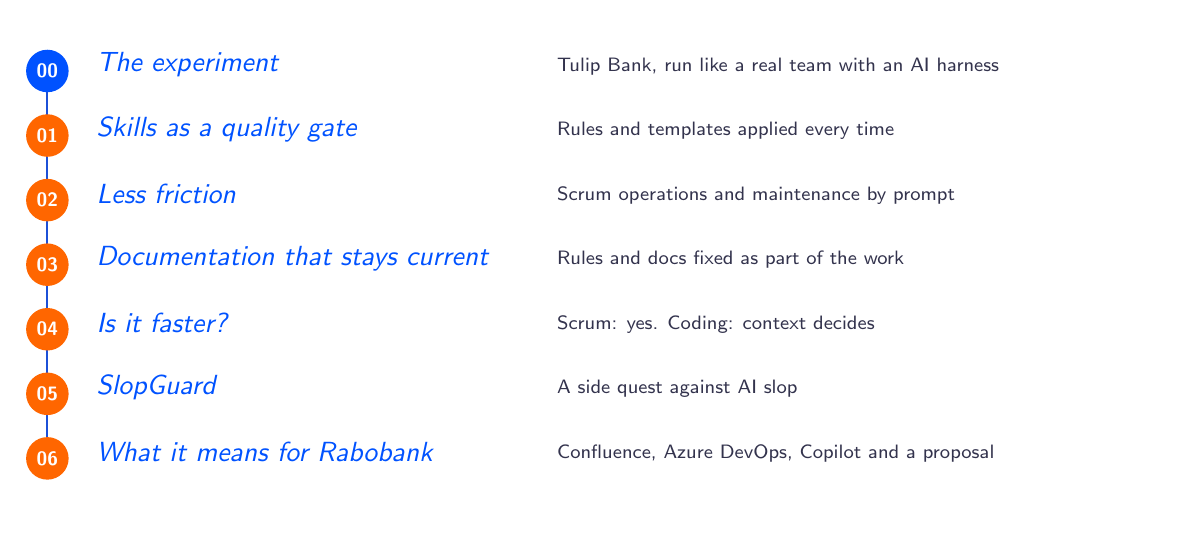
\begin{tikzpicture}
  \useasboundingbox (0,0) rectangle (14.4,6.1);
  \draw[line] (0.25,5.5) -- (0.25,0.55);
  \fill[raboLine] (0.25,5.72) circle (2pt);
  \foreach \n/\t/\s [count=\i] in {
    0/The experiment/{Tulip Bank, run like a real team with an AI harness},
    1/Skills as a quality gate/Rules and templates applied every time,
    2/Less friction/Scrum operations and maintenance by prompt,
    3/Documentation that stays current/Rules and docs fixed as part of the work,
    4/Is it faster?/Scrum: yes. Coding: context decides,
    5/SlopGuard/A side quest against AI slop,
    6/What it means for Rabobank/{Confluence, Azure DevOps, Copilot and a proposal}}{
    \pgfmathsetmacro{\y}{5.55-(\i-1)*0.82}
    \ifnum\i=1 \def\c{raboBlue}\else\def\c{raboOrange}\fi
    \fill[\c] (0.25,\y) circle (0.27);
    \node[text=white,font=\scriptsize\bfseries] at (0.25,\y) {0\n};
    \node[anchor=west,font=\normalsize\itshape,text=raboBlue] at (0.75,\y+0.08) {\t};
    \node[anchor=west,font=\scriptsize,text=raboInk] at (6.6,\y+0.06) {\s};
  }
\end{tikzpicture}
\end{frame}

% ================================================================ 0 experiment
\section{The experiment}

\begin{frame}[t]{Tulip Bank: a dummy project, run like a real team}{The experiment}
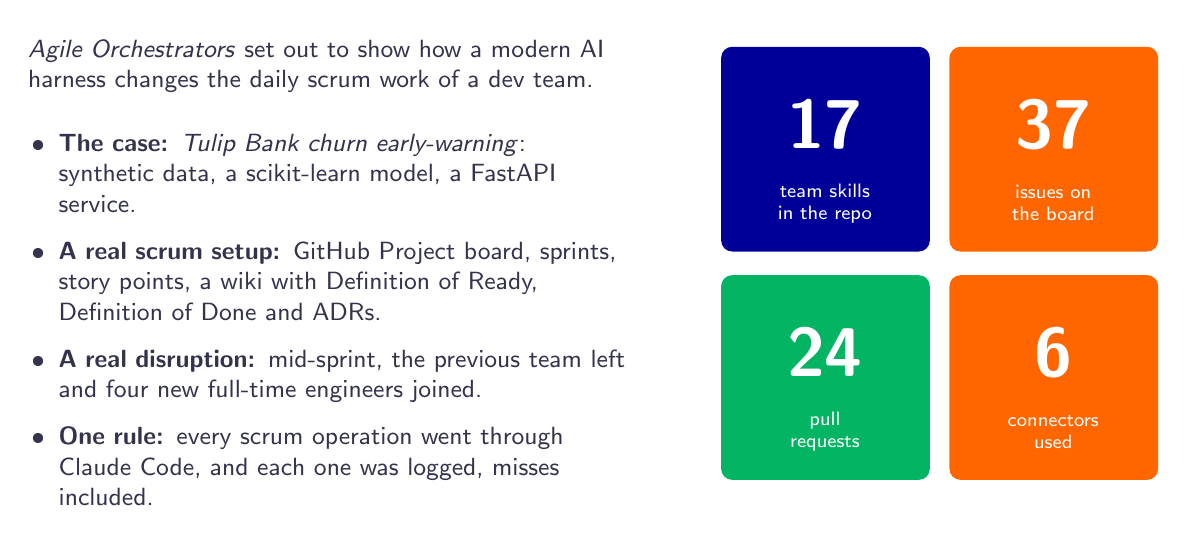
\begin{tikzpicture}
  \useasboundingbox (0,0) rectangle (14.4,6.1);
  \node[body,text width=7.6cm,font=\small] at (0,5.95) {%
    \textit{Agile Orchestrators} set out to show how a modern AI harness changes the daily
    scrum work of a dev team.\par\medskip
    \begin{itemize}\setlength{\itemsep}{4pt}
      \item \textbf{The case:} \emph{Tulip Bank churn early-warning}: synthetic data,
        a scikit-learn model, a FastAPI service.
      \item \textbf{A real scrum setup:} GitHub Project board, sprints, story points,
        a wiki with Definition of Ready, Definition of Done and ADRs.
      \item \textbf{A real disruption:} mid-sprint, the previous team left and
        four new full-time engineers joined.
      \item \textbf{One rule:} every scrum operation went through Claude Code, and
        each one was logged, misses included.
    \end{itemize}};
  \foreach \x/\y/\num/\lab/\sty in {
      8.8/3.25/17/team skills\\in the repo/nbox,
      11.7/3.25/37/issues on\\the board/obox,
      8.8/0.35/24/pull\\requests/gbox,
      11.7/0.35/6/connectors\\used/obox}{
    \node[\sty,minimum width=2.65cm,minimum height=2.6cm,anchor=south west] at (\x,\y) {};
    \node[text=white,font=\fontsize{30}{30}\selectfont\bfseries] at (\x+1.325,\y+1.62) {\num};
    \node[text=white,font=\scriptsize,align=center] at (\x+1.325,\y+0.62) {\lab};
  }
\end{tikzpicture}
\end{frame}


\begin{frame}[t]{One track through the whole scrum lifecycle}{The experiment \,\textperiodcentered\, skills in the repo}
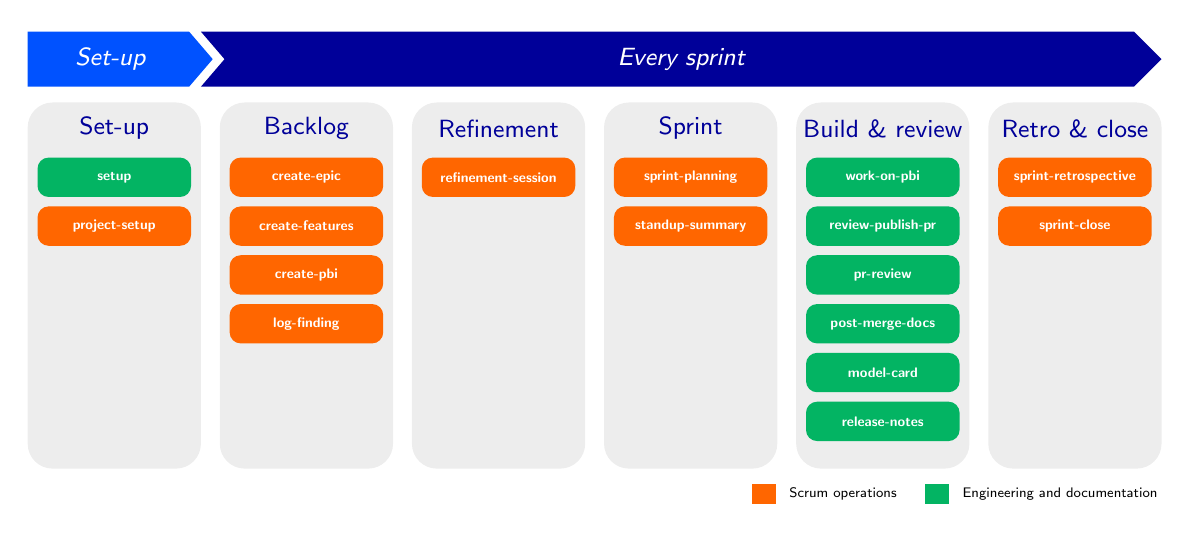
\begin{tikzpicture}
  \useasboundingbox (0,0) rectangle (14.4,6.1);
  % chevron band (reference slide 3)
  \fill[raboBlue] (0,5.35) -- (2.05,5.35) -- (2.35,5.7) -- (2.05,6.05) -- (0,6.05) -- cycle;
  \node[text=white,font=\small\itshape] at (1.05,5.7) {Set-up};
  \fill[raboNavy] (2.2,5.35) -- (14.05,5.35) -- (14.4,5.7) -- (14.05,6.05) -- (2.2,6.05)
    -- (2.5,5.7) -- cycle;
  \node[text=white,font=\small\itshape] at (8.3,5.7) {Every sprint};
  % columns
  \foreach \x/\h [count=\i] in {0/Set-up,2.44/Backlog,4.88/Refinement,7.32/Sprint,
      9.76/Build \& review,12.2/Retro \& close}{
    \fill[panel] (\x,0.5) rectangle (\x+2.2,5.15);
    \node[font=\small,text=raboNavy] at (\x+1.1,4.82) {\h};
  }
  \skb{gbox}{0}{4.2}{setup}
  \skb{obox}{0}{3.58}{project-setup}
  \skb{obox}{2.44}{4.2}{create-epic}
  \skb{obox}{2.44}{3.58}{create-features}
  \skb{obox}{2.44}{2.96}{create-pbi}
  \skb{obox}{2.44}{2.34}{log-finding}
  \skb{obox}{4.88}{4.2}{refinement-session}
  \skb{obox}{7.32}{4.2}{sprint-planning}
  \skb{obox}{7.32}{3.58}{standup-summary}
  \skb{gbox}{9.76}{4.2}{work-on-pbi}
  \skb{gbox}{9.76}{3.58}{review-publish-pr}
  \skb{gbox}{9.76}{2.96}{pr-review}
  \skb{gbox}{9.76}{2.34}{post-merge-docs}
  \skb{gbox}{9.76}{1.72}{model-card}
  \skb{gbox}{9.76}{1.10}{release-notes}
  \skb{obox}{12.2}{4.2}{sprint-retrospective}
  \skb{obox}{12.2}{3.58}{sprint-close}
  % legend
  \fill[raboOrange] (9.2,0.05) rectangle (9.5,0.3);
  \node[anchor=west,font=\tiny] at (9.55,0.175) {Scrum operations};
  \fill[raboGreen] (11.4,0.05) rectangle (11.7,0.3);
  \node[anchor=west,font=\tiny] at (11.75,0.175) {Engineering and documentation};
\end{tikzpicture}
\end{frame}

% ================================================================ 1 skills
\section{Skills as a quality gate}

\begin{frame}[t]{Discipline moves from people into the skill}{Skills as a quality gate}
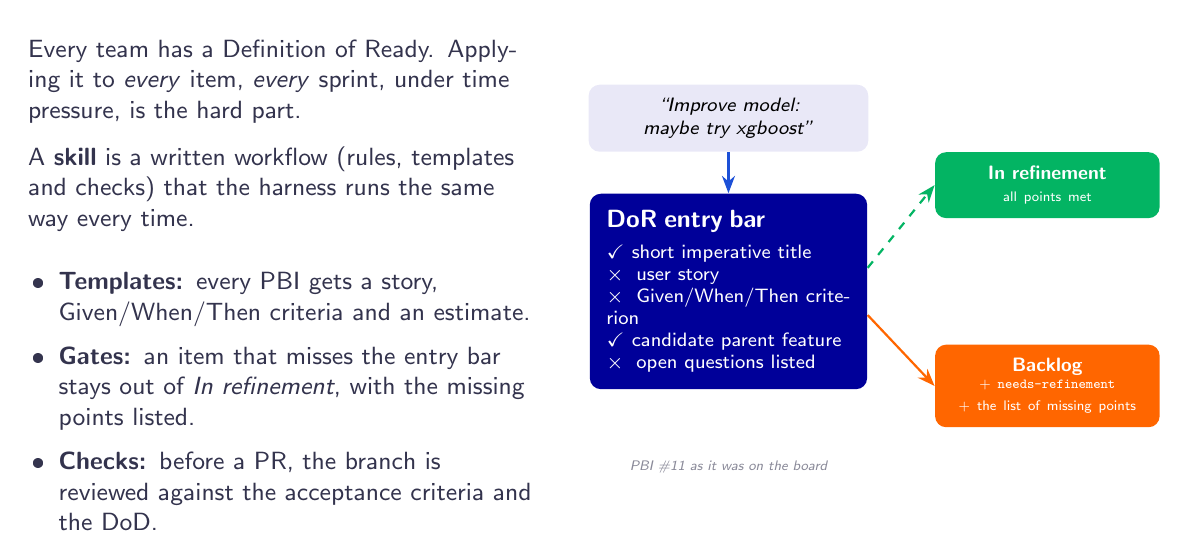
\begin{tikzpicture}
  \useasboundingbox (0,0) rectangle (14.4,6.1);
  \node[body,text width=6.4cm,font=\small] at (0,5.95) {%
    Every team has a Definition of Ready. Applying it to \emph{every} item, \emph{every}
    sprint, under time pressure, is the hard part.\par\medskip
    A \textbf{skill} is a written workflow (rules, templates and checks) that the
    harness runs the same way every time.\par\medskip
    \begin{itemize}\setlength{\itemsep}{3pt}
      \item \textbf{Templates:} every PBI gets a story, Given\slash When\slash Then
        criteria and an estimate.
      \item \textbf{Gates:} an item that misses the entry bar stays out of
        \emph{In refinement}, with the missing points listed.
      \item \textbf{Checks:} before a PR, the branch is reviewed against the
        acceptance criteria and the DoD.
    \end{itemize}};
  % gate diagram
  \node[fill=raboLilac,rounded corners=4pt,font=\scriptsize\itshape,text width=3.2cm,
    align=center,inner sep=5pt] (in) at (8.9,4.95) {``Improve model:\\maybe try xgboost''};
  \node[nbox,text width=3.1cm,inner sep=6pt,align=left] (gate) at (8.9,2.75) {%
    {\small\bfseries DoR entry bar}\\[3pt]
    $\checkmark$ short imperative title\\
    $\times$\; user story\\
    $\times$\; Given\slash When\slash Then criterion\\
    $\checkmark$ candidate parent feature\\
    $\times$\; open questions listed};
  \draw[arr] (in) -- (gate);
  \node[gbox,text width=2.5cm,inner sep=5pt] (ok) at (12.95,4.1)
    {\textbf{In refinement}\\\tiny all points met};
  \node[obox,text width=2.5cm,inner sep=5pt] (ko) at (12.95,1.55)
    {\textbf{Backlog}\\\tiny + \texttt{needs-refinement}\\ + the list of missing points};
  \draw[arr,raboGreen,dashed] (gate.east) ++(0,0.3) -- (ok.west);
  \draw[arr,raboOrange] (gate.east) ++(0,-0.3) -- (ko.west);
  \node[font=\tiny\itshape,text=raboMuted,anchor=north] at (8.9,0.72)
    {PBI \#11 as it was on the board};
\end{tikzpicture}
\end{frame}

\begin{frame}[t]{Quality went up on every step of scrum}{Skills as a quality gate \,\textperiodcentered\, examples from the log}
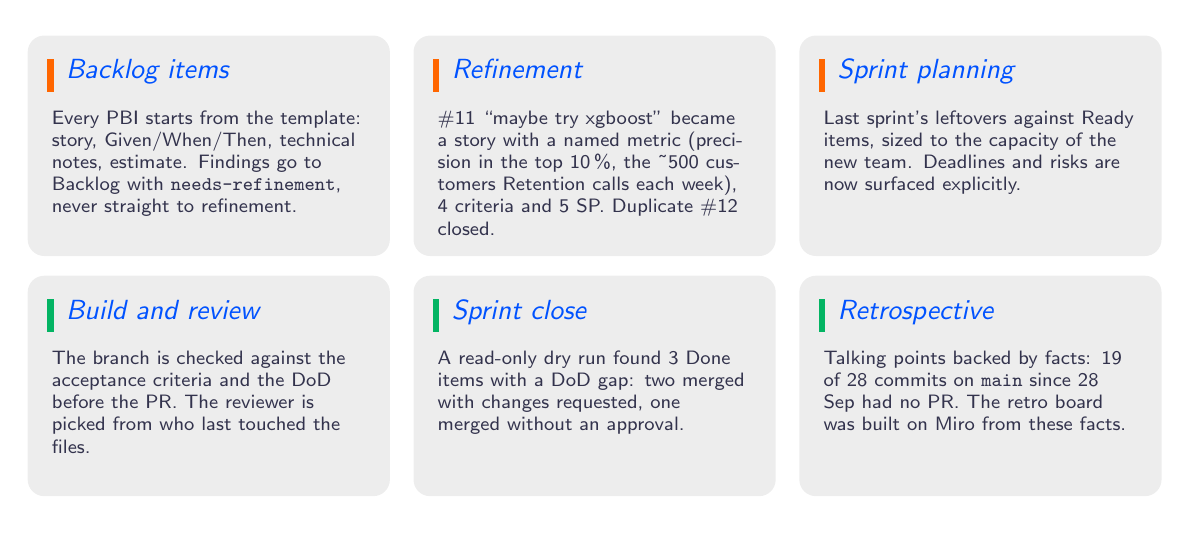
\begin{tikzpicture}
  \useasboundingbox (0,0) rectangle (14.4,6.1);
  \foreach \x/\y/\c/\t/\d in {
    0/6.0/raboOrange/Backlog items/{Every PBI starts from the template: story, Given\slash When\slash Then,
      technical notes, estimate. Findings go to Backlog with \texttt{needs-refinement}, never
      straight to refinement.},
    4.9/6.0/raboOrange/Refinement/{\#11 ``maybe try xgboost'' became a story with a named metric
      (precision in the top 10\,\%, the \textasciitilde500 customers Retention calls each week),
      4 criteria and 5 SP. Duplicate \#12 closed.},
    9.8/6.0/raboOrange/Sprint planning/{Last sprint's leftovers against Ready items, sized to the
      capacity of the new team. Deadlines and risks are now surfaced explicitly.},
    0/2.95/raboGreen/Build and review/{The branch is checked against the acceptance criteria and
      the DoD before the PR. The reviewer is picked from who last touched the files.},
    4.9/2.95/raboGreen/Sprint close/{A read-only dry run found 3 Done items with a DoD gap:
      two merged with changes requested, one merged without an approval.},
    9.8/2.95/raboGreen/Retrospective/{Talking points backed by facts: 19 of 28 commits on
      \texttt{main} since 28 Sep had no PR. The retro board was built on Miro from these facts.}}{
    \fill[raboPanel,rounded corners=6pt] (\x,\y) rectangle (\x+4.6,\y-2.8);
    \fill[\c] (\x+0.25,\y-0.3) rectangle (\x+0.33,\y-0.72);
    \node[htitle,font=\normalsize\itshape] at (\x+0.48,\y-0.3) {\t};
    \node[body,text width=3.95cm] at (\x+0.3,\y-0.95) {\d};
  }
\end{tikzpicture}
\end{frame}


% ================================================================ 2 friction
\section{Less friction}

\begin{frame}[t]{Scrum operations by prompt}{Less friction \,\textperiodcentered\, what the PO typed and what the harness did}
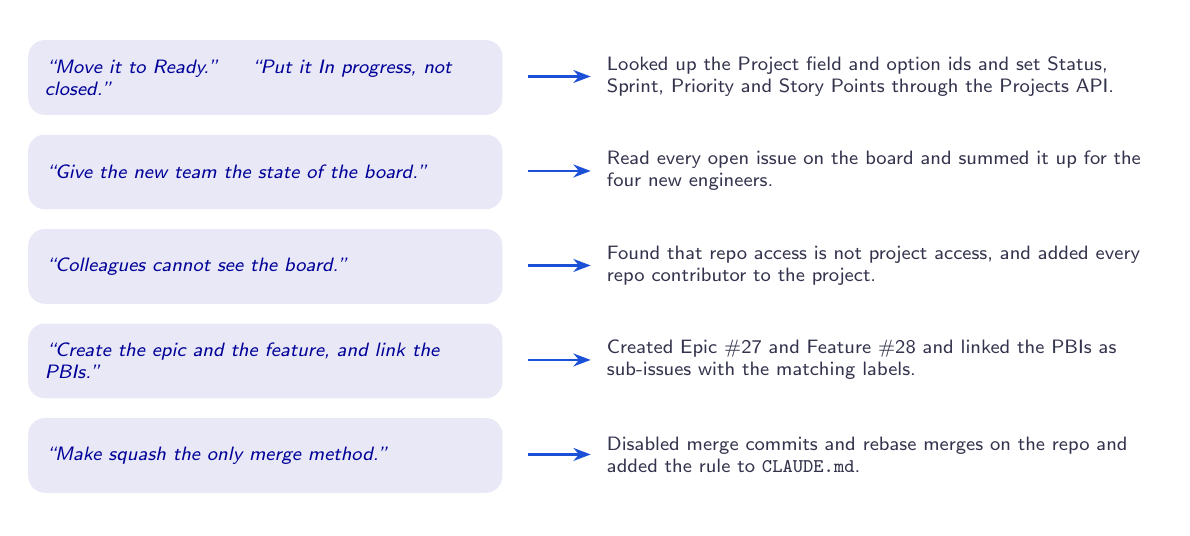
\begin{tikzpicture}
  \useasboundingbox (0,0) rectangle (14.4,6.1);
  \foreach \q/\a [count=\i] in {
    {``Move it to Ready.'' \quad ``Put it In progress, not closed.''}/
      {Looked up the Project field and option ids and set Status, Sprint, Priority and
      Story Points through the Projects API.},
    {``Give the new team the state of the board.''}/
      Read every open issue on the board and summed it up for the four new engineers.,
    {``Colleagues cannot see the board.''}/
      {Found that repo access is not project access, and added every repo contributor
      to the project.},
    {``Create the epic and the feature, and link the PBIs.''}/
      Created Epic \#27 and Feature \#28 and linked the PBIs as sub-issues with the matching
      labels.,
    {``Make squash the only merge method.''}/
      {Disabled merge commits and rebase merges on the repo and added the rule to
      \texttt{CLAUDE.md}.}}{
    \pgfmathsetmacro{\y}{5.95-(\i-1)*1.2}
    \node[fill=raboLilac,rounded corners=6pt,text width=5.6cm,font=\scriptsize\itshape,
      text=raboNavy,anchor=north west,inner sep=6pt,minimum height=0.95cm] (q\i) at (0,\y) {\q};
    \draw[arr] (6.35,\y-0.47) -- (7.15,\y-0.47);
    \node[body,text width=7.0cm,anchor=west] at (7.35,\y-0.47) {\a};
  }
\end{tikzpicture}
\end{frame}


\begin{frame}[t]{Friction removed, control kept}{Less friction \,\textperiodcentered\, who does what}
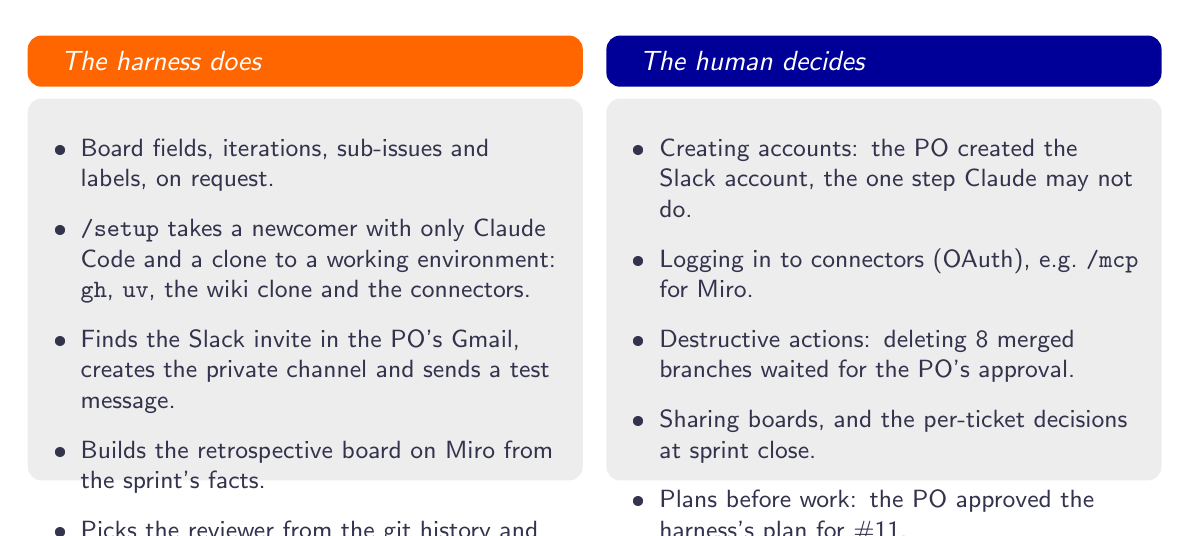
\begin{tikzpicture}
  \useasboundingbox (0,0) rectangle (14.4,6.1);
  \foreach \x/\c/\h/\items in {
    0/raboOrange/The harness does/{
      \item Board fields, iterations, sub-issues and labels, on request.
      \item \sk{/setup} takes a newcomer with only Claude Code and a clone to a working
        environment: \texttt{gh}, \texttt{uv}, the wiki clone and the connectors.
      \item Finds the Slack invite in the PO's Gmail, creates the private channel and
        sends a test message.
      \item Builds the retrospective board on Miro from the sprint's facts.
      \item Picks the reviewer from the git history and requests the review.},
    7.35/raboNavy/The human decides/{
      \item Creating accounts: the PO created the Slack account, the one step Claude
        may not do.
      \item Logging in to connectors (OAuth), e.g.\ \sk{/mcp} for Miro.
      \item Destructive actions: deleting 8 merged branches waited for the PO's
        approval.
      \item Sharing boards, and the per-ticket decisions at sprint close.
      \item Plans before work: the PO approved the harness's plan for \#11.}}{
    \fill[\c,rounded corners=5pt] (\x,6.0) rectangle (\x+7.05,5.35);
    \node[anchor=west,text=white,font=\normalsize\itshape] at (\x+0.3,5.675) {\h};
    \fill[raboPanel,rounded corners=5pt] (\x,5.2) rectangle (\x+7.05,0.35);
    \node[body,text width=6.5cm,font=\small] at (\x+0.28,5.0)
      {\begin{itemize}\setlength{\itemsep}{5pt}\items\end{itemize}};
  }
\end{tikzpicture}
\end{frame}

% ================================================================ 3 documentation
\section{Documentation that stays current}

\begin{frame}[t]{Rules and docs are fixed as part of the work}{Documentation that stays current}
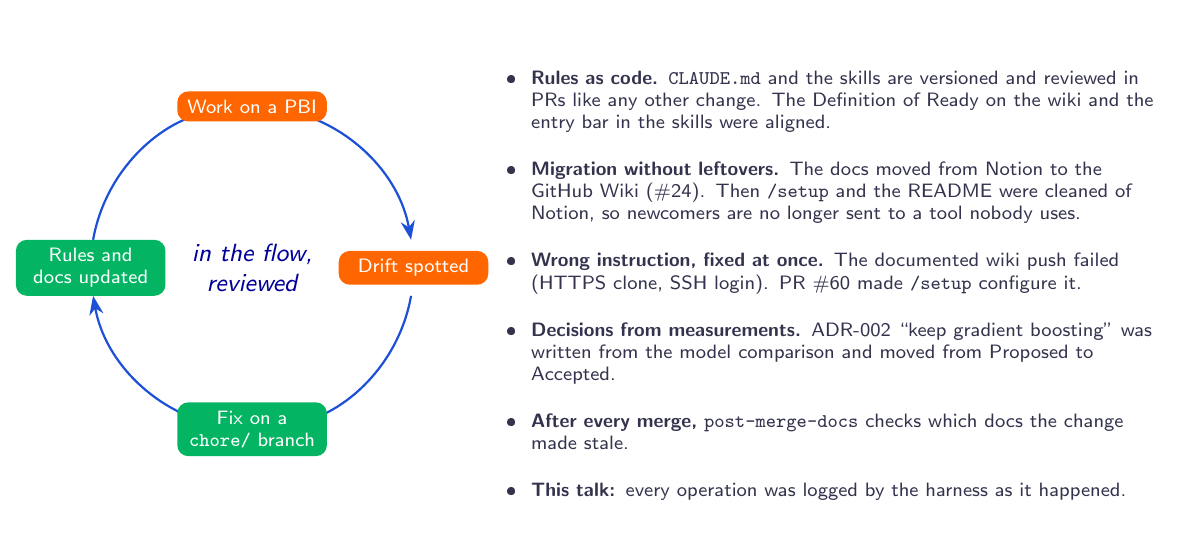
\begin{tikzpicture}
  \useasboundingbox (0,0) rectangle (14.4,6.1);
  % cycle
  \coordinate (c) at (2.85,3.05);
  \draw[raboLine,line width=0.8pt,-{Stealth[length=2.4mm]}] ($(c)+(80:2.05)$)
    arc[start angle=80,end angle=10,radius=2.05];
  \draw[raboLine,line width=0.8pt,-{Stealth[length=2.4mm]}] ($(c)+(-10:2.05)$)
    arc[start angle=-10,end angle=-80,radius=2.05];
  \draw[raboLine,line width=0.8pt,-{Stealth[length=2.4mm]}] ($(c)+(-100:2.05)$)
    arc[start angle=-100,end angle=-170,radius=2.05];
  \draw[raboLine,line width=0.8pt,-{Stealth[length=2.4mm]}] ($(c)+(170:2.05)$)
    arc[start angle=170,end angle=100,radius=2.05];
  \node[obox,minimum width=1.9cm] at ($(c)+(90:2.05)$) {Work on a PBI};
  \node[obox,minimum width=1.9cm] at ($(c)+(0:2.05)$) {Drift spotted};
  \node[gbox,minimum width=1.9cm] at ($(c)+(-90:2.05)$) {Fix on a\\\texttt{chore/} branch};
  \node[gbox,minimum width=1.9cm] at ($(c)+(180:2.05)$) {Rules and\\docs updated};
  \node[font=\small\itshape,text=raboNavy,align=center] at (c) {in the flow,\\reviewed};
  % bullets
  \node[body,text width=8.4cm,font=\scriptsize] at (6.0,5.95) {%
    \begin{itemize}\setlength{\itemsep}{5pt}
      \item \textbf{Rules as code.} \texttt{CLAUDE.md} and the skills are versioned and
        reviewed in PRs like any other change. The Definition of Ready on the wiki and the
        entry bar in the skills were aligned.
      \item \textbf{Migration without leftovers.} The docs moved from Notion to the GitHub Wiki
        (\#24). Then \sk{/setup} and the README were cleaned of Notion, so newcomers are no
        longer sent to a tool nobody uses.
      \item \textbf{Wrong instruction, fixed at once.} The documented wiki push failed (HTTPS
        clone, SSH login). PR \#60 made \sk{/setup} configure it.
      \item \textbf{Decisions from measurements.} ADR-002 ``keep gradient boosting'' was
        written from the model comparison and moved from Proposed to Accepted.
      \item \textbf{After every merge,} \sk{post-merge-docs} checks which docs the change made
        stale.
      \item \textbf{This talk:} every operation was logged by the harness as it happened.
    \end{itemize}};
\end{tikzpicture}
\end{frame}

% ================================================================ 4 faster?
\section{Is it faster?}

\begin{frame}[t]{Faster? An honest answer}{Is it faster?}
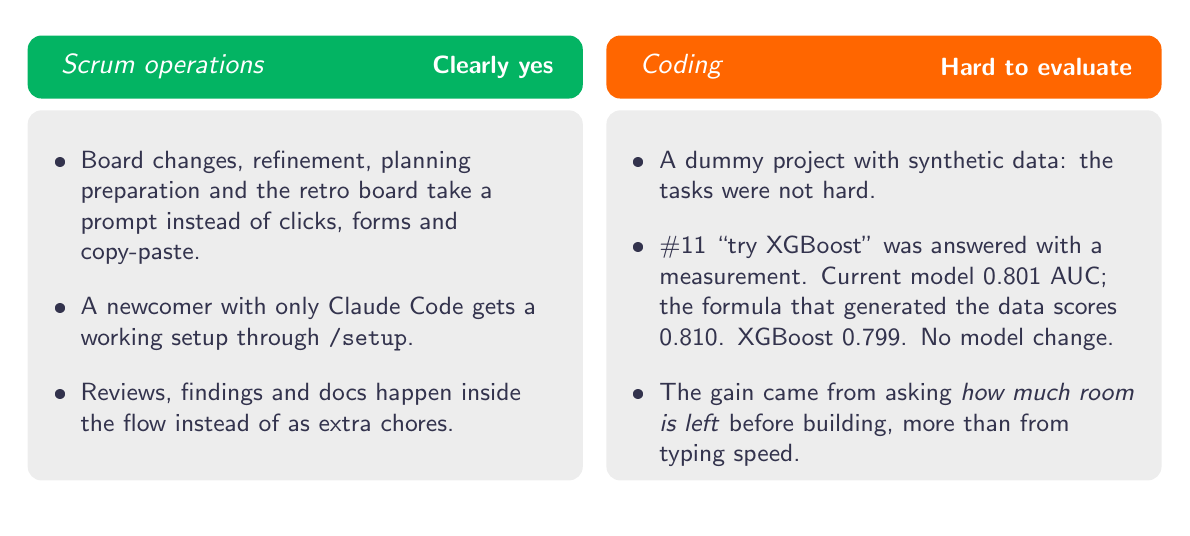
\begin{tikzpicture}
  \useasboundingbox (0,0) rectangle (14.4,6.1);
  \foreach \x/\c/\h/\v/\items in {
    0/raboGreen/Scrum operations/Clearly yes/{
      \item Board changes, refinement, planning preparation and the retro board take a
        prompt instead of clicks, forms and copy-paste.
      \item A newcomer with only Claude Code gets a working setup through \sk{/setup}.
      \item Reviews, findings and docs happen inside the flow instead of as extra chores.},
    7.35/raboOrange/Coding/Hard to evaluate/{
      \item A dummy project with synthetic data: the tasks were not hard.
      \item \#11 ``try XGBoost'' was answered with a measurement. Current model 0.801 AUC;
        the formula that generated the data scores 0.810. XGBoost 0.799. No model change.
      \item The gain came from asking \emph{how much room is left} before building, more than
        from typing speed.}}{
    \fill[\c,rounded corners=5pt] (\x,6.0) rectangle (\x+7.05,5.2);
    \node[anchor=west,text=white,font=\normalsize\itshape] at (\x+0.3,5.6) {\h};
    \node[anchor=east,text=white,font=\small\bfseries] at (\x+6.8,5.6) {\v};
    \fill[raboPanel,rounded corners=5pt] (\x,5.05) rectangle (\x+7.05,0.35);
    \node[body,text width=6.5cm,font=\small] at (\x+0.28,4.85)
      {\begin{itemize}\setlength{\itemsep}{7pt}\items\end{itemize}};
  }
\end{tikzpicture}
\end{frame}

\begin{frame}[t]{The real multiplier is context}{Is it faster? \,\textperiodcentered\, our hypothesis}
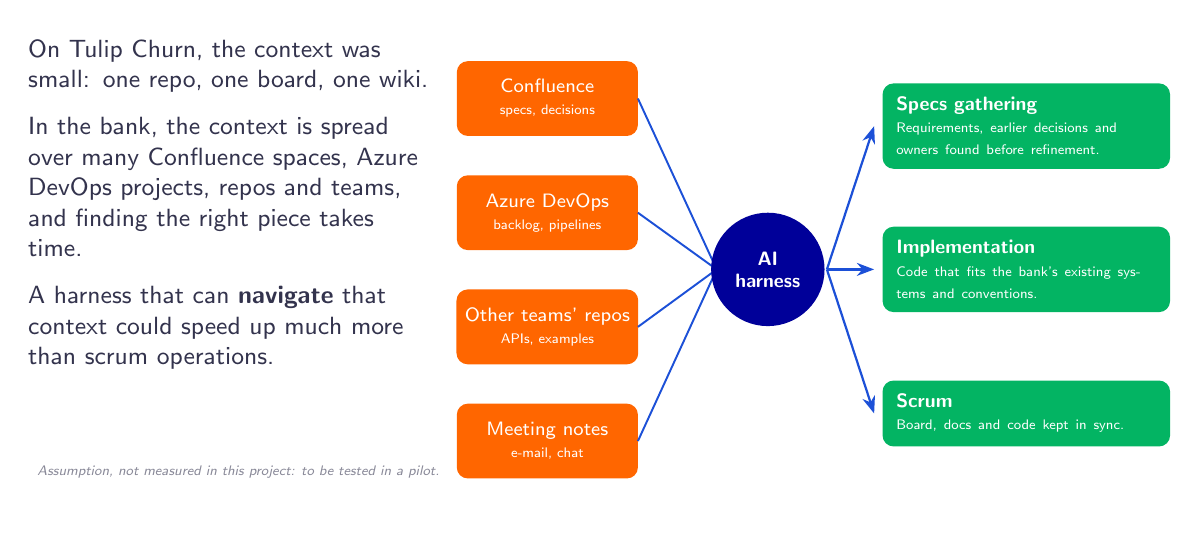
\begin{tikzpicture}
  \useasboundingbox (0,0) rectangle (14.4,6.1);
  \node[body,text width=5.1cm,font=\small] at (0,5.95) {%
    On Tulip Churn, the context was small: one repo, one board, one wiki.\par\medskip
    In the bank, the context is spread over many Confluence spaces, Azure DevOps projects,
    repos and teams, and finding the right piece takes time.\par\medskip
    A harness that can \textbf{navigate} that context could speed up much more than
    scrum operations.};
  \node[font=\tiny\itshape,text=raboMuted,anchor=south west] at (0,0.25)
    {Assumption, not measured in this project: to be tested in a pilot.};
  % context sources -> harness -> outcomes
  \foreach \t/\y/\s in {{Confluence\\\tiny specs, decisions}/5.2/obox,
      {Azure DevOps\\\tiny backlog, pipelines}/3.75/obox,
      {Other teams' repos\\\tiny APIs, examples}/2.3/obox,
      {Meeting notes\\\tiny e-mail, chat}/0.85/obox}{
    \node[\s,minimum width=2.3cm,minimum height=0.95cm] at (6.6,\y) {\t};
    \draw[line] (7.75,\y) -- (8.75,3.03);
  }
  \fill[raboNavy] (9.4,3.03) circle (0.72);
  \node[text=white,font=\scriptsize\bfseries,align=center] at (9.4,3.03) {AI\\harness};
  \foreach \t/\d/\y in {Specs gathering/{Requirements, earlier decisions and owners found
      before refinement.}/4.85,
    Implementation/Code that fits the bank's existing systems and conventions./3.03,
    Scrum/{Board, docs and code kept in sync.}/1.2}{
    \draw[arr] (10.15,3.03) -- (10.75,\y);
    \node[gbox,minimum width=3.4cm,text width=3.3cm,align=left,anchor=west,inner sep=5pt]
      at (10.85,\y) {\textbf{\t}\\\tiny \d};
  }
\end{tikzpicture}
\end{frame}

% ================================================================ 5 slopguard
\section{SlopGuard}

\begin{frame}[t]{AI writes code fast, and slop piles up just as fast}{SlopGuard \,\textperiodcentered\, the problem}
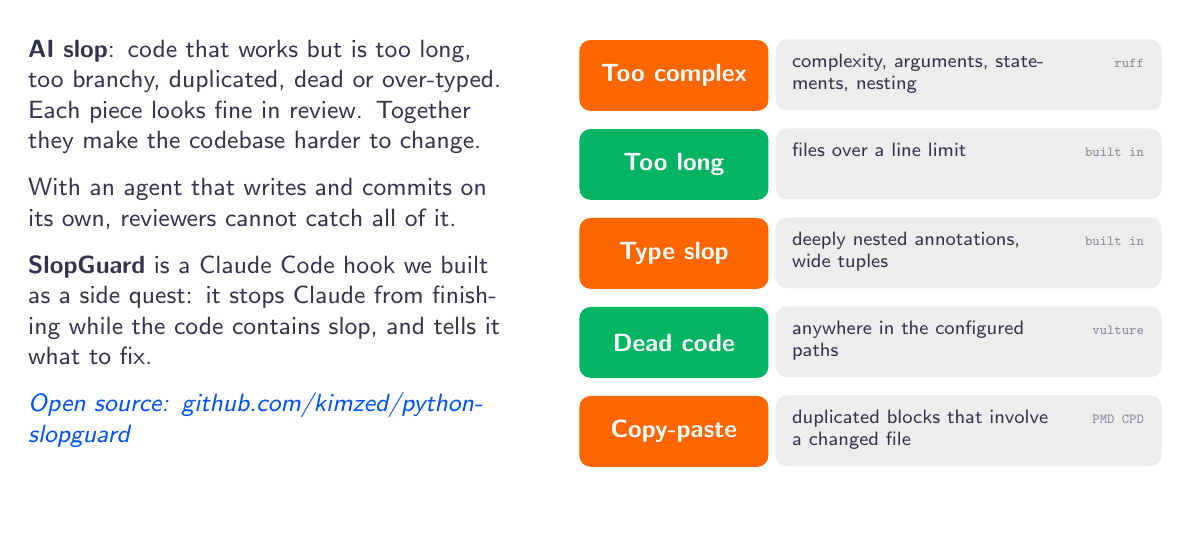
\begin{tikzpicture}
  \useasboundingbox (0,0) rectangle (14.4,6.1);
  \node[body,text width=6.2cm,font=\small] at (0,5.95) {%
    \textbf{AI slop}: code that works but is too long, too branchy, duplicated, dead or
    over-typed. Each piece looks fine in review. Together they make the codebase harder
    to change.\par\medskip
    With an agent that writes and commits on its own, reviewers cannot catch all of it.
    \par\medskip
    \textbf{SlopGuard} is a Claude Code hook we built as a side quest: it stops Claude from
    finishing while the code contains slop, and tells it what to fix.\par\medskip
    {\color{raboBlue}\itshape Open source: github.com/kimzed/python-slopguard}};
  \foreach \t/\d/\tool/\c [count=\i] in {
      Too complex/{complexity, arguments, statements, nesting}/ruff/obox,
      Too long/files over a line limit/built in/gbox,
      Type slop/{deeply nested annotations, wide tuples}/built in/obox,
      Dead code/anywhere in the configured paths/vulture/gbox,
      Copy-paste/duplicated blocks that involve a changed file/PMD CPD/obox}{
    \pgfmathsetmacro{\y}{5.95-(\i-1)*1.13}
    \node[\c,anchor=north west,minimum width=2.4cm,minimum height=0.9cm,font=\small\bfseries]
      at (7.0,\y) {\t};
    \fill[raboPanel,rounded corners=4pt] (9.5,\y) rectangle (14.4,\y-0.9);
    \node[body,text width=3.4cm] at (9.7,\y-0.18) {\d};
    \node[anchor=north east,font=\tiny\ttfamily,text=raboMuted] at (14.3,\y-0.12) {\tool};
  }
\end{tikzpicture}
\end{frame}


\begin{frame}[t]{What dogfooding SlopGuard taught us}{SlopGuard \,\textperiodcentered\, lessons from PBI \#11}
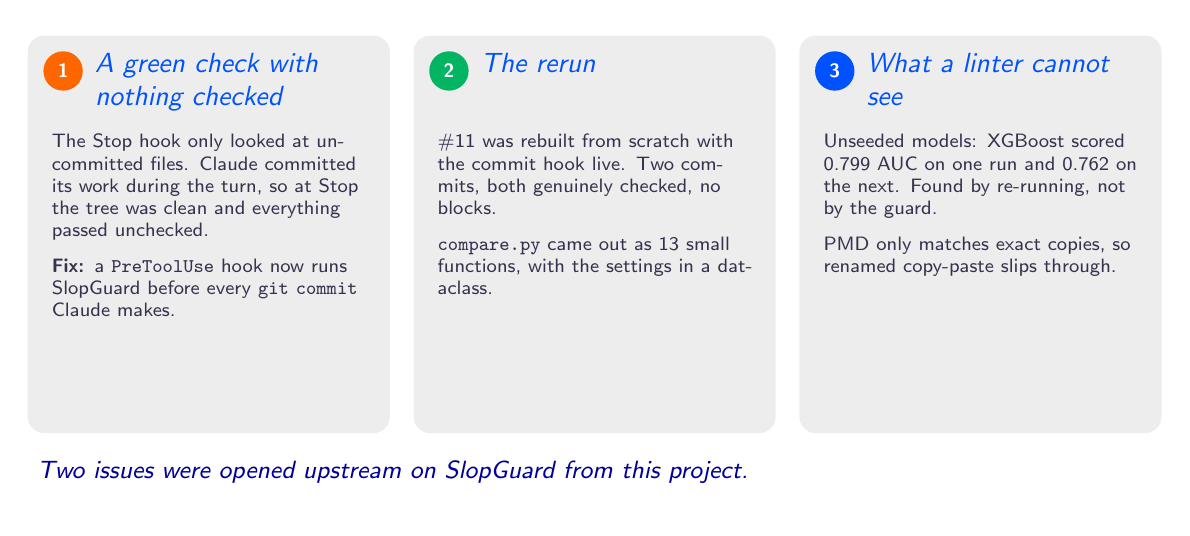
\begin{tikzpicture}
  \useasboundingbox (0,0) rectangle (14.4,6.1);
  \foreach \x/\c/\n/\t/\d in {
    0/raboOrange/1/A green check with nothing checked/{The Stop hook only looked at
      uncommitted files. Claude committed its work during the turn, so at Stop the tree was
      clean and everything passed unchecked.\\[5pt]
      \textbf{Fix:} a \texttt{PreToolUse} hook now runs SlopGuard before every
      \texttt{git commit} Claude makes.},
    4.9/raboGreen/2/The rerun/{\#11 was rebuilt from scratch with the commit hook live.
      Two commits, both genuinely checked, no blocks.\\[5pt]
      \texttt{compare.py} came out as 13 small functions, with the settings in a
      dataclass.},
    9.8/raboBlue/3/What a linter cannot see/{Unseeded models: XGBoost scored 0.799 AUC on one
      run and 0.762 on the next. Found by re-running, not by the guard.\\[5pt]
      PMD only matches exact copies, so renamed copy-paste slips through.}}{
    \fill[raboPanel,rounded corners=6pt] (\x,6.0) rectangle (\x+4.6,0.95);
    \fill[\c] (\x+0.45,5.55) circle (0.25);
    \node[text=white,font=\scriptsize\bfseries] at (\x+0.45,5.55) {\n};
    \node[htitle,text width=3.6cm,font=\normalsize\itshape] at (\x+0.85,5.78) {\t};
    \node[body,text width=4.0cm] at (\x+0.3,4.75) {\d};
  }
  \node[font=\small\itshape,text=raboNavy,anchor=west] at (0,0.45)
    {Two issues were opened upstream on SlopGuard from this project.};
\end{tikzpicture}
\end{frame}

% ================================================================ 6 rabobank
\section{What it means for Rabobank}

\begin{frame}[t]{Our tools at the bank do not talk to each other yet}{What it means for Rabobank}
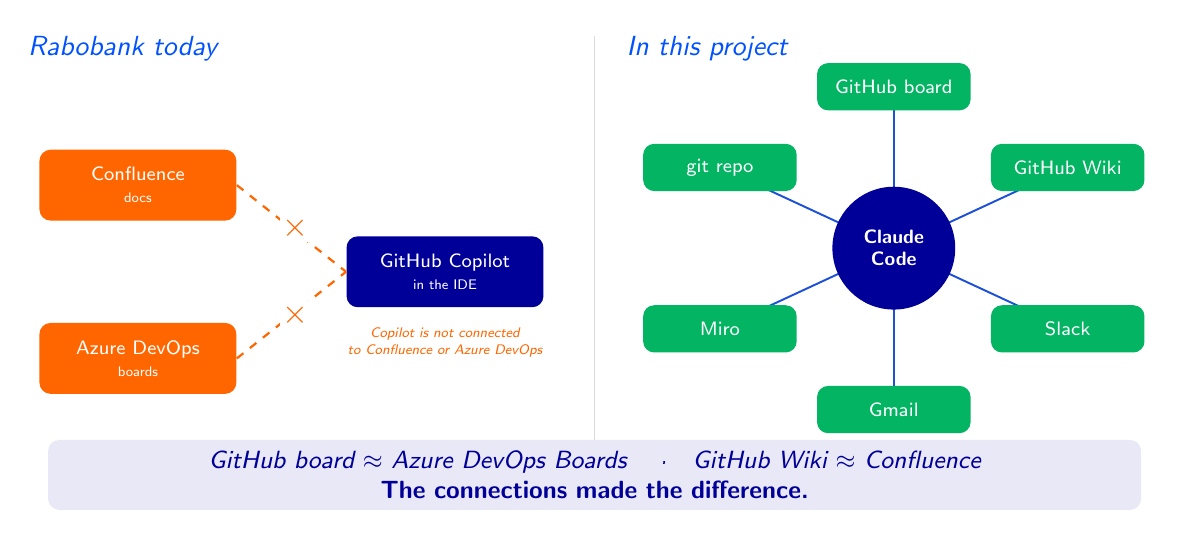
\begin{tikzpicture}
  \useasboundingbox (0,0) rectangle (14.4,6.1);
  % left: rabo today
  \node[htitle,font=\normalsize\itshape] at (0,6.0) {Rabobank today};
  \node[obox,minimum width=2.5cm,minimum height=0.9cm] (conf) at (1.4,4.1) {Confluence\\\tiny docs};
  \node[obox,minimum width=2.5cm,minimum height=0.9cm] (ado) at (1.4,1.9) {Azure DevOps\\\tiny boards};
  \node[nbox,minimum width=2.5cm,minimum height=0.9cm] (cop) at (5.3,3.0)
    {GitHub Copilot\\\tiny in the IDE};
  \draw[raboOrange,line width=0.8pt,dashed] (conf.east) -- (cop.west);
  \draw[raboOrange,line width=0.8pt,dashed] (ado.east) -- (cop.west);
  \foreach \y in {3.55,2.45}{
    \node[fill=white,text=raboOrange,font=\large\bfseries,inner sep=1pt] at (3.4,\y) {$\times$};
  }
  \node[font=\tiny\itshape,text=raboOrange,align=center] at (5.3,2.1)
    {Copilot is not connected\\to Confluence or Azure DevOps};
  \draw[raboGrey,line width=0.6pt] (7.2,0.4) -- (7.2,6.0);
  % right: this project
  \node[htitle,font=\normalsize\itshape] at (7.6,6.0) {In this project};
  \coordinate (h) at (11.0,3.3);
  \foreach \a/\t in {90/GitHub board,30/GitHub Wiki,-30/Slack,-90/Gmail,210/Miro,150/git repo}{
    \draw[line] (h) -- ($(h)+(\a:2.55 and 2.05)$);
    \node[gbox,minimum width=1.95cm,minimum height=0.6cm] at ($(h)+(\a:2.55 and 2.05)$) {\t};
  }
  \fill[raboNavy] (h) circle (0.78);
  \node[text=white,font=\scriptsize\bfseries,align=center] at (h) {Claude\\Code};
  \node[fill=raboLilac,rounded corners=4pt,text width=13.6cm,align=center,
    font=\small\itshape,text=raboNavy,inner sep=4pt] at (7.2,0.42)
    {GitHub board $\approx$ Azure DevOps Boards \quad\textperiodcentered\quad GitHub Wiki
     $\approx$ Confluence\\ \upshape\bfseries The connections made the difference.};
\end{tikzpicture}
\end{frame}

\begin{frame}[t]{Proposal: bring the harness to a Rabobank team}{What it means for Rabobank \,\textperiodcentered\, to discuss}
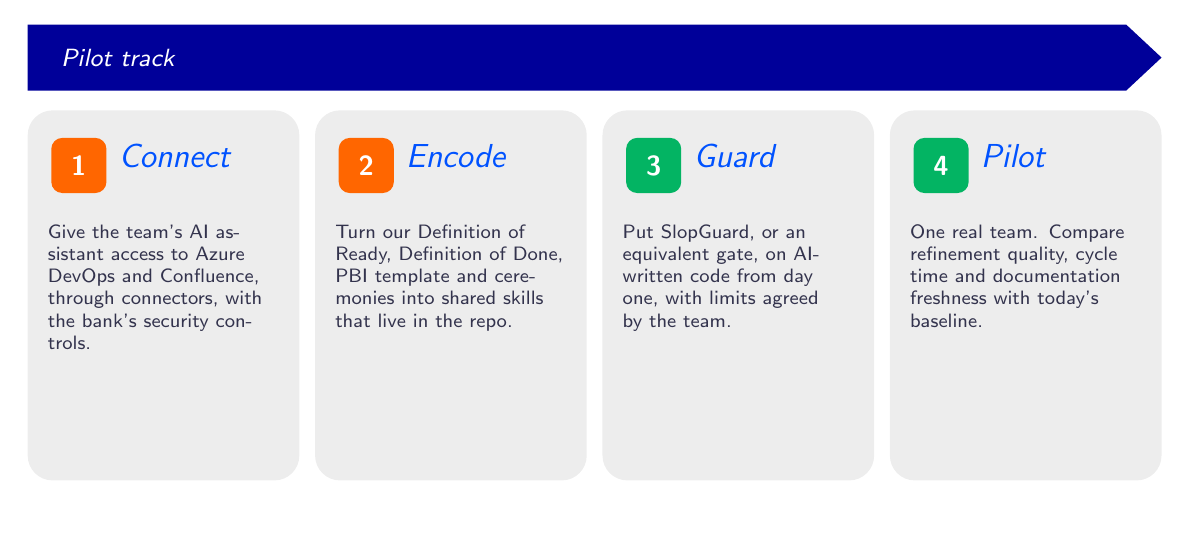
\begin{tikzpicture}
  \useasboundingbox (0,0) rectangle (14.4,6.1);
  \fill[raboNavy] (0,5.3) -- (13.95,5.3) -- (14.4,5.72) -- (13.95,6.14) -- (0,6.14) -- cycle;
  \node[anchor=west,text=white,font=\small\itshape] at (0.3,5.72) {Pilot track};
  \foreach \x/\n/\t/\d/\c in {
    0/1/Connect/{Give the team's AI assistant access to Azure DevOps and Confluence,
      through connectors, with the bank's security controls.}/obox,
    3.65/2/Encode/{Turn our Definition of Ready, Definition of Done, PBI template and
      ceremonies into shared skills that live in the repo.}/obox,
    7.3/3/Guard/{Put SlopGuard, or an equivalent gate, on AI-written code from day one,
      with limits agreed by the team.}/gbox,
    10.95/4/Pilot/{One real team. Compare refinement quality, cycle time and documentation
      freshness with today's baseline.}/gbox}{
    \fill[panel] (\x,5.05) rectangle (\x+3.45,0.35);
    \node[\c,minimum width=0.7cm,minimum height=0.7cm,font=\normalsize\bfseries]
      at (\x+0.65,4.35) {\n};
    \node[htitle,font=\large\itshape] at (\x+1.15,4.62) {\t};
    \node[body,text width=2.95cm,font=\scriptsize] at (\x+0.25,3.6) {\d};
  }
\end{tikzpicture}
\end{frame}


\begin{frame}[t]{Takeaways}{Agile Orchestrators}
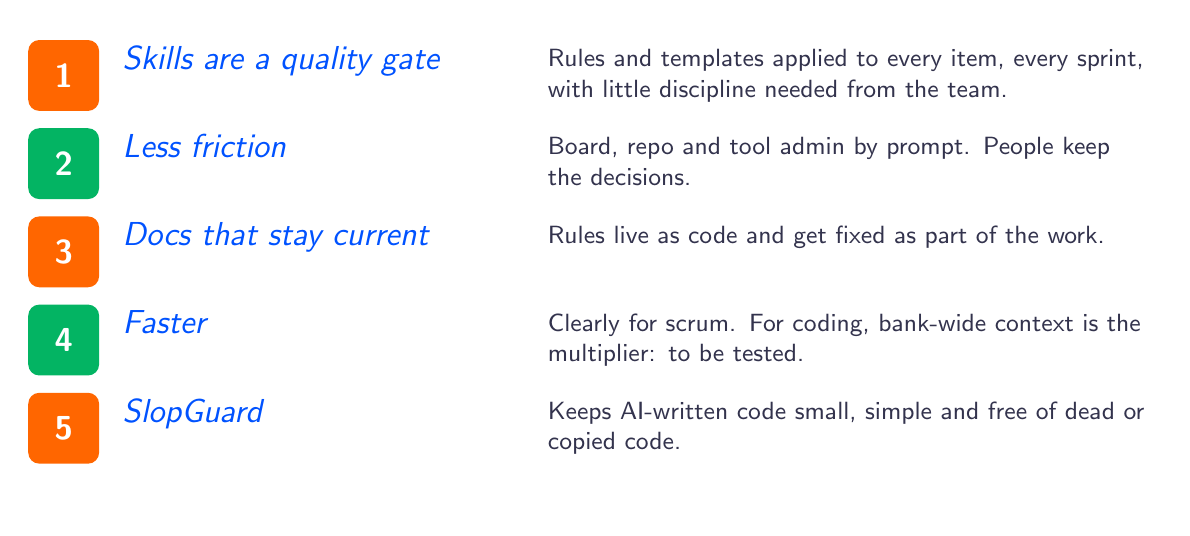
\begin{tikzpicture}
  \useasboundingbox (0,0) rectangle (14.4,6.1);
  \foreach \t/\d/\c [count=\i] in {
    Skills are a quality gate/{Rules and templates applied to every item, every sprint, with
      little discipline needed from the team.}/obox,
    Less friction/{Board, repo and tool admin by prompt. People keep the decisions.}/gbox,
    Docs that stay current/Rules live as code and get fixed as part of the work./obox,
    Faster/{Clearly for scrum. For coding, bank-wide context is the multiplier:
      to be tested.}/gbox,
    SlopGuard/{Keeps AI-written code small, simple and free of dead or copied code.}/obox}{
    \pgfmathsetmacro{\y}{5.95-(\i-1)*1.12}
    \node[\c,anchor=north west,minimum width=0.9cm,minimum height=0.9cm,
      font=\large\bfseries] at (0,\y) {\i};
    \node[htitle,font=\large\itshape] at (1.2,\y-0.08) {\t};
    \node[body,text width=7.6cm,font=\small] at (6.6,\y-0.12) {\d};
  }
\end{tikzpicture}
\end{frame}

% ================================================================ closing
{\setbeamertemplate{background}{%
  \begin{tikzpicture}
    \useasboundingbox (0,0) rectangle (16,9);
    \fill[raboNavy] (0,4.30) rectangle (9.9,5.45);
    \node[anchor=west,text=white,font=\fontsize{26}{28}\selectfont] at (0.8,4.86) {Questions?};
    \fill[raboOrange,rounded corners=5pt] (3.5,2.85) rectangle (9.9,4.10);
    \node[anchor=west,text=white,font=\small\bfseries\itshape,text width=6.0cm,align=left]
      at (3.7,3.47) {Thank you from\\Team Agile Orchestrators};
    \node[anchor=west,text=raboMuted,font=\small] at (3.55,2.30)
      {Repo, board, wiki and the harness log are open to browse};
    \connectorring{12.55}{5.75}{2.05}
    \node[align=center,font=\footnotesize,text=raboNavy] at (12.55,5.95)
      {\textbf{\large Claude Code}\\[1pt] {\scriptsize AGILE ORCHESTRATORS}};
    \node[rotate=8,font=\small\itshape\bfseries,text=raboOrange] at (12.7,5.15)
      {Join the sprint};
    \node[anchor=south east,inner sep=0] at (15.6,0.35)
      {
\includegraphics[height=1.35cm]{rabobank-logo}};
  \end{tikzpicture}}
 \begin{frame}[plain]\mbox{}\end{frame}}

\end{document}
